\section{Casi d'Uso}\label{CasiUso}
\subsection{Introduzione}\label{CasiUso_Introduzione}
Nella seguente sezione verranno identificati i casi d'uso che abbiamo individuato.\\
Il numero di casi che abbiamo analizzato è limitato poiché il plug-in fornisce funzionalità aggiuntive ad una piattaforma preesistente, per la quale non è fornita documentazione in quanto già disponibile presso il sito web del fornitore della piattaforma: \textit{Grafana Labs}.

\subsection{Attori}\label{Attori}
È importante notare che il numero esiguo di differenti attori che possono approcciarsi al prodotto in esame è principalmente dovuto al fatto che, essendo il progetto \textit{G\&B} un plug-in di un sistema indipendente, poche tipologie di utenti possono effettivamente approcciarsi al prodotto finale.\\
È altrettanto importante sottolineare che il sistema di registrazione ed autenticazione dell'utente viene gestito interamente dal sistema \textit{Grafana}, dal momento che, ovviamente, il prodotto finale non avrà una funzionalità di autenticazione interna.

\subsubsection*{Attori Primari}
\begin{itemize}
\item \textbf{Utente:} si riferisce ad un generico utente che ha effettuato l'autenticazione al sistema \textit{Grafana}. È l'unica tipologia di utente con facoltà di interagire con il prodotto, in quanto questo risulta essere un plug-in.
\end{itemize}

\subsubsection*{Attori Secondari}
\begin{itemize}
\item \textbf{Piattaforma \textit{Grafana}:} sistema di monitoraggio di flusso dati, di cui il prodotto da realizzare è un plug-in. Consente agli utenti autenticati, attraverso funzionalità proprie, di realizzare grafici ed alert riferiti a dati forniti dal plug-in.
\end{itemize}

\begin{comment}
\begin{itemize}
	\item \textbf{Attore Primario:}
	\item \textbf{Precondizioni:}
	\begin{enumerate}
 		\item
	\end{enumerate}
	\item \textbf{Postcondizioni:}
	\begin{enumerate}
		\item
	\end{enumerate}
	\item \textbf{Scenario Principale:}
	\begin{enumerate}
		\item
	\end{enumerate}
	\item \textbf{Estensioni:}
\end{itemize}
\end{comment}

%PANORAMICA UC
\begin{comment} 
\pagebreak

\subsection{Panoramica Casi d'Uso}\label{PanoramicaUC}
Questa sezione ha l'obiettivo di presentare una vista generale dei casi d'uso fondamentali del plug-in al fine di fornire una comprensione generale del prodotto migliore e più immediata. I casi d'uso sono stati suddivisi in due diagrammi separati per agevolarne la facilità di comprensione, anche e soprattutto a livello visivo.\\
Il primo diagramma (\hyperref[Panoramica UC Configurazione]{Panoramica UC Configurazione (§\ref*{Panoramica UC Configurazione})}) racchiude i casi d'uso atti a modellare le operazioni che devono essere eseguite dall'utente prima di poter avviare il monitoraggio dei dati. Il secondo diagramma (\hyperref[Panoramica UC Monitoraggio]{Panoramica UC Monitoraggio (§\ref*{Panoramica UC Monitoraggio})}) invece contiene principalmente i casi d'uso che modellano la gestione dei monitoraggi che utilizzano le reti bayesiane.

\begin{figure}[H]
	\begin{center}
		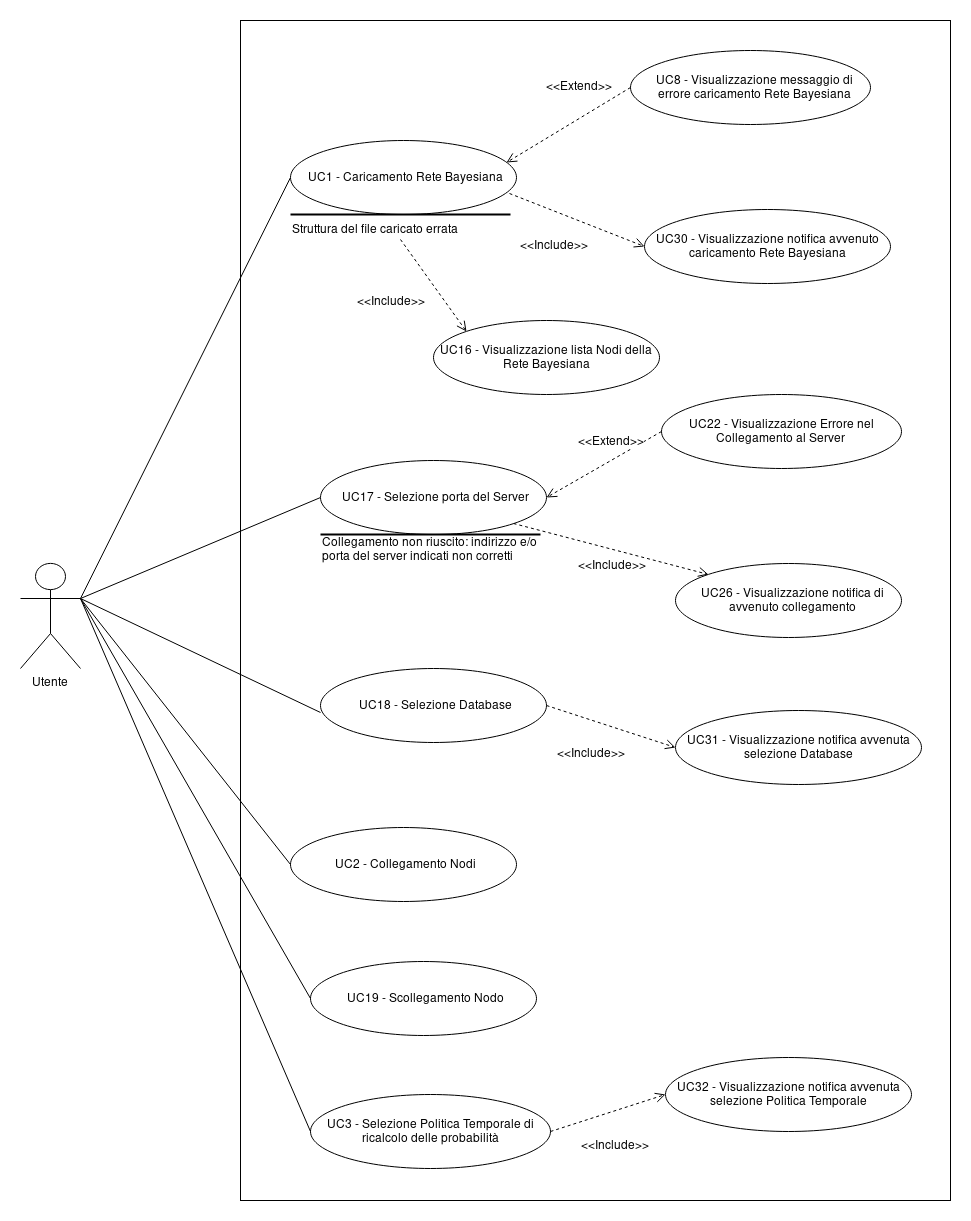
\includegraphics[scale=0.4]{./images/VistaUC.png}
		 \caption{Panoramica dei Casi d'Uso di configurazione delle impostazioni di collegamento}
		 \label{Panoramica UC Configurazione}
	\end{center}
\end{figure}

\pagebreak

\begin{figure}[H]
	\begin{center}
		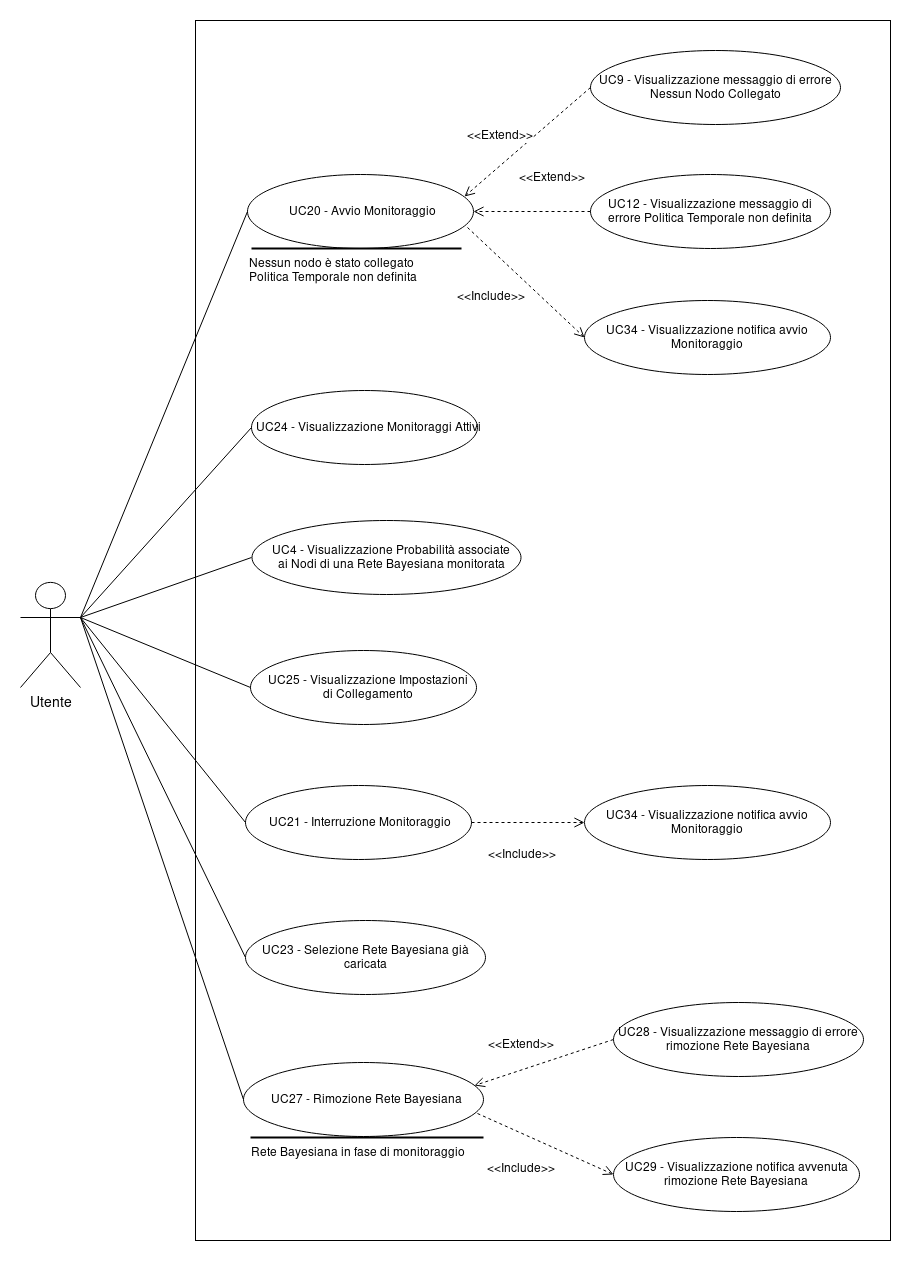
\includegraphics[scale=0.4]{./images/VistaUC2.png}
		 \caption{Panoramica dei Casi d'Uso di gestione dei monitoraggi che utilizzano le reti bayesiane}
		 \label{Panoramica UC Monitoraggio}
	\end{center}
\end{figure}

\pagebreak
\end{comment}
%FINE PANORAMICA UC

\pagebreak
\subsection{UC1 - Caricamento Rete Bayesiana}\label{UC1}
\begin{figure}[H]
	\begin{center}
		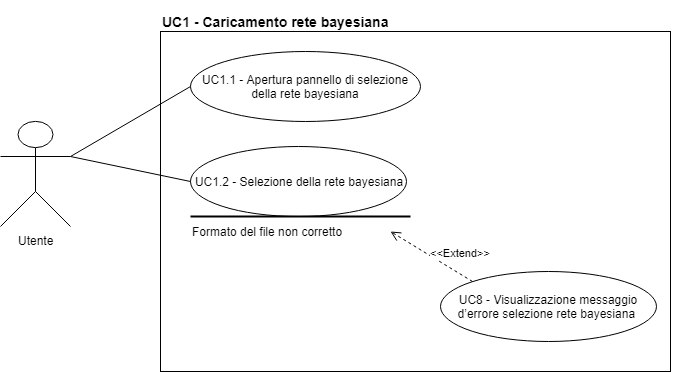
\includegraphics[scale=0.5]{./images/UC1.png}
		 \caption{UC1 - Aggiunta della Rete Bayesiana al Plug-in G\&B}
	\end{center}
\end{figure}

\begin{itemize}
	\item \textbf{Attore Primario}: Utente;
	\item \textbf{Precondizioni}:
		\begin{enumerate}
			\item L'utente deve aver effettuato il login nella piattaforma \textit{Grafana}, deve aver selezionato una dashboard e aggiunto il pannello \textit{G\&B};
			\item L'utente deve aver correttamente configurato la connessione al server (\hyperref[UC17]{UC17 (§\ref*{UC17})}).
		\end{enumerate}
	\item \textbf{Postcondizioni}:
	\begin{enumerate}
		\item L'utente ha aggiunto la rete bayesiana al plug-in;
		\item L'utente visualizza il pulsante denominato "Avvio Monitoraggio";
		\item Nel caso in cui l'utente stesse precedentemente visualizzando le impostazioni di monitoraggio di un'altra rete queste vengono salvate nel server, se la rete non era in monitoraggio, e ne vengono sostituite da quelle della nuova rete, che l'utente andrà a definire.
	\end{enumerate}
	\item \textbf{Scenario Principale:}
	\begin{enumerate}
		\item (\hyperref[UC1.1]{UC1.1 (§\ref*{UC1.1})}) L'utente apre il pannello di selezione della rete bayesiana da caricare attraverso il click del pulsante "Seleziona Rete";
		\item (\hyperref[UC1.2]{UC1.2 (§\ref*{UC1.2})}) L'utente seleziona la rete bayesiana che desidera caricare.
	\end{enumerate}
	\item \textbf{Estensioni:} \hyperref[UC8]{UC8 (§\ref*{UC8})} estende \hyperref[UC1.2]{UC1.2 (§\ref*{UC1.2})}: l'utente visualizza un messaggio di errore nel caso in cui l'operazione non sia andata a buon fine.
	\item \textbf{Inclusioni:} 
	\begin{enumerate}
		\item UC1 include \hyperref[UC30]{UC30 (§\ref*{UC30})}: Viene visualizzata una notifica di avvenuto collegamento;
		\item UC1 include \hyperref[UC16]{UC16 (§\ref*{UC16})}: Viene visualizzata la lista di nodi di cui la rete bayesiana caricata è costituita.
	\end{enumerate}
\end{itemize}

\pagebreak

\subsubsection{UC1.1 - Apertura Pannello di Selezione del File}\label{UC1.1}
\begin{itemize}
	\item \textbf{Attore Primario}: Utente;
	\item \textbf{Precondizioni}: l'utente visualizza il pannello \textit{G\&B} nella dashboard;
	\item \textbf{Postcondizioni}: l'utente ha cliccato il bottone con etichetta "Seleziona Rete" e visualizza il pannello per la selezione del file della rete;
	\item \textbf{Scenario Principale}: l'utente clicca il pulsante con etichetta "Seleziona Rete".
\end{itemize}


\subsubsection{UC1.2 - Selezione della Rete Bayesiana}\label{UC1.2}
\begin{itemize}
	\item \textbf{Attore Primario}: Utente;
	\item \textbf{Precondizioni}: l'utente ha cliccato il bottone con etichetta "Seleziona Rete";
	\item \textbf{Postcondizioni}: l'utente ha caricato con successo il file \textit{JSON} contente la definizione della rete bayesiana;
	\item \textbf{Scenario Principale}:
	\begin{enumerate}
		\item L'utente seleziona dalla finestra il file da importare;
		\item L'utente clicca il pulsante con etichetta "Apri".
	\end{enumerate}
	\item \textbf{Estensioni:} \hyperref[UC8]{UC8 (§\ref*{UC8})}: l'utente visualizza un messaggio di errore nel caso in cui l'operazione di caricamento del file non sia andata a buon fine.
\end{itemize}

\pagebreak

\subsection{UC2 - Collegamento Nodi al Flusso Dati}\label{UC2}
\begin{figure}[H]
\centering
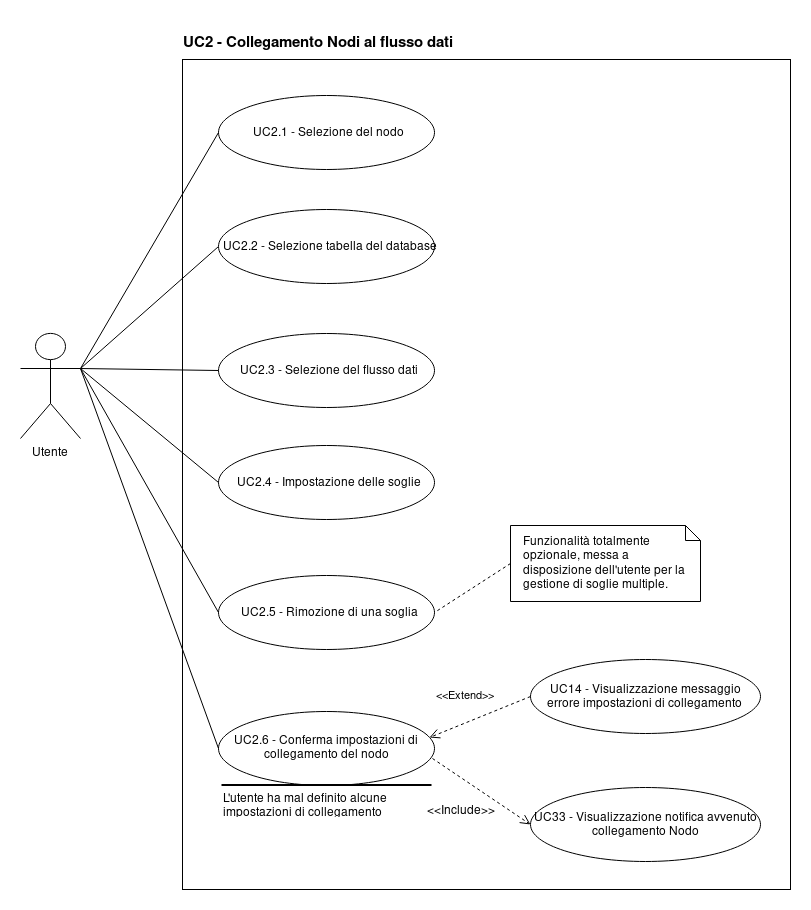
\includegraphics[scale=0.5]{./images/UC2.png}
\caption{UC2 - Collegamento Nodi al Flusso Dati}
\end{figure}

\begin{itemize}
\item \textbf{Attore Primario}: Utente;
\item \textbf{Precondizioni}:
\begin{enumerate}
	\item L'utente ha caricato con successo la rete bayesiana (\hyperref[UC1]{UC1(§\ref*{UC1})});
	\item L'utente visualizza la lista di nodi di cui la rete bayesiana è costituita	(\hyperref[UC16]{UC16 (§\ref*{UC16})}).
\end{enumerate}
\item \textbf{Postcondizione}: L'utente ha collegato correttamente uno o più nodi ad un flusso dati, definendone le soglie per i rispettivi stati;
\item \textbf{Scenario Principale}:
 \begin{enumerate}
 \item (\hyperref[UC2.1]{UC2.1 (§\ref*{UC2.1})}) Selezione del Nodo;
 \item (\hyperref[UC2.2]{UC2.2 (§\ref*{UC2.2})}) Selezione della tabella del database;
 \item (\hyperref[UC2.3]{UC2.3 (§\ref*{UC2.3})}) Selezione del flusso dati;
 \item (\hyperref[UC2.4]{UC2.4 (§\ref*{UC2.4})}) Impostazione delle soglie;
 \item (\hyperref[UC2.5]{UC2.5 (§\ref*{UC2.5})}) Rimozione di una soglia;
 \item (\hyperref[UC2.6]{UC2.6 (§\ref*{UC2.6})}) Conferma impostazioni di collegamento del nodo.
 \end{enumerate}
\item \textbf{Estensioni:} \hyperref[UC14]{UC14 (§\ref*{UC14})} estende \hyperref[UC2.6]{UC2.6 (§\ref*{UC2.6})}: l'utente visualizza un messaggio di errore nel caso in cui non abbia definito correttamente le impostazioni di collegamento;
\item \textbf{Inclusioni:} \hyperref[UC2.6]{UC2.6 (§\ref*{UC2.6})} include \hyperref[UC33]{UC33 (§\ref*{UC33})}: Visualizzazione notifica avvenuto collegamento nodo.
\end{itemize}

\pagebreak

\subsubsection{UC2.1 - Selezione del Nodo}\label{UC2.1}
\begin{itemize}
\item \textbf{Attore Primario:} Utente;
\item \textbf{Precondizione:} l'utente visualizza la lista di nodi di cui la rete bayesiana è costituita ed il 	corrispondente stato (\hyperref[UC16]{UC16 (§\ref*{UC16})});
\item \textbf{Postcondizione:} l'utente visualizza una finestra contenente le impostazioni di collegamento del nodo selezionato;
\item \textbf{Scenario Principale:} l'utente clicca il nominativo del nodo che desidera collegare al flusso dati.
\end{itemize}

\subsubsection{UC2.2 - Selezione Tabella Database}\label{UC2.2}
\begin{itemize}
\item \textbf{Attore Primario:} Utente;
\item \textbf{Precondizione:} l'utente ha selezionato il nodo che desidera collegare al flusso dati 					(\hyperref[UC2.1]{UC2.1 (§\ref*{UC2.1})});
\item \textbf{Postcondizioni:}
	\begin{enumerate}
	\item L'utente ha selezionato la tabella del database contente i flussi dati da selezionare;
	\item In base alla tabella selezionata cambia contestualemnte il contenuto del menù a tendina per la selezione del flusso dati (\hyperref[UC2.3]{UC2.3 (§\ref*{UC2.3})});
	\end{enumerate}
\item \textbf{Scenario Principale:} l'utente seleziona, attraverso un menù a tendina, il flusso dati a cui desidera collegare il nodo in esame.
\end{itemize}

\subsubsection{UC2.3 - Selezione del Flusso Dati}\label{UC2.3}
\begin{itemize}
	\item \textbf{Attore Primario:} Utente;
	\item \textbf{Precondizione:} l'utente ha selezionato il nodo che desidera collegare al flusso dati 						(\hyperref[UC2.1]{UC2.1 (§\ref*{UC2.1})});
	\item \textbf{Postcondizioni:} l'utente ha selezionato il flusso dati a cui collegare il nodo desiderato;
	\item \textbf{Scenario Principale:} l'utente seleziona, attraverso un menù a tendina, il flusso dati a cui desidera collegare il nodo in esame.
\end{itemize}

\pagebreak

\subsubsection{UC2.4 - Impostazione Soglie}\label{UC2.4}

\begin{figure}[H]
\centering
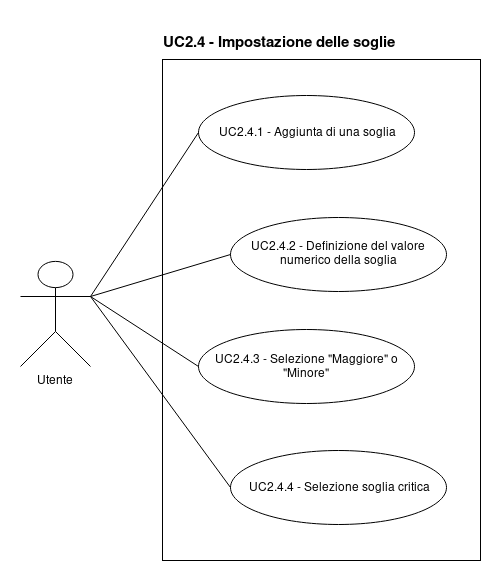
\includegraphics[scale=0.5]{./images/UC2-4.png}
\caption{UC2.4 - Impostazione delle soglie}
\end{figure}

\begin{itemize}
\item \textbf{Attore Primario:} Utente;
\item \textbf{Precondizione:} l'utente ha selezionato il nodo che desidera collegare al flusso dati 					(\hyperref[UC2.1]{UC2.1 (§\ref*{UC2.1})});
\item \textbf{Postcondizione:} l'utente ha impostato, per ogni stato del nodo, una o più soglie, le quali hanno la funzionalità di definire gli insiemi di valori per i quali la probabilità associata allo stato in questione risulta pari al 100\%, mentre le probabilità associate agli altri stati risultano pari allo 0\%;
\item \textbf{Scenario Principale:}
	\begin{enumerate}
	\item (\hyperref[UC2.4.1]{UC2.4.1 (§\ref*{UC2.4.1})}) Aggiunta di una soglia;
	\item (\hyperref[UC2.4.2]{UC2.4.2 (§\ref*{UC2.4.2})}) Definizione del valore numerico della soglia;
	\item (\hyperref[UC2.4.3]{UC2.4.3 (§\ref*{UC2.4.3})}) Selezione segno della soglia;
	\item (\hyperref[UC2.4.4]{UC2.4.4 (§\ref*{UC2.4.4})}) Selezione soglia critica;
	\item (\hyperref[UC2.4.5]{UC2.4.5 (§\ref*{UC2.4.5})}) Selezione "<=" come verso della soglia;
	\item (\hyperref[UC2.4.6]{UC2.4.6 (§\ref*{UC2.4.6})}) Selezione "<" come verso della soglia;
	\item (\hyperref[UC2.4.7]{UC2.4.7 (§\ref*{UC2.4.7})}) Selezione ">=" come verso della soglia;
	\item (\hyperref[UC2.4.8]{UC2.4.8 (§\ref*{UC2.4.8})}) Selezione ">" come verso della soglia.
	\end{enumerate}
\end{itemize}

\paragraph{UC2.4.1 - Aggiunta di una Soglia}\label{UC2.4.1}
\begin{itemize}
	\item \textbf{Attore Primario:} Utente;
	\item \textbf{Precondizioni:} l'utente ha selezionato il nodo che desidera collegare al flusso dati 					(\hyperref[UC2.1]{UC2.1 (§\ref*{UC2.1})});
	\item \textbf{Postcondizione:} l'utente visualizza i campi dati editabili da compilare per definire una soglia per lo stato in questione;
	\item \textbf{Scenario Principale:} l'utente aggiunge una soglia editabile per lo stato del nodo desiderato cliccando il pulsante "Aggiungi Soglia" posizionato accanto al nominativo dello stato. Se lo desidera l'utente può ripetere più volte l'operazione per lo stesso stato, aggiungendo così la possibilità di definire molteplici soglie per lo stesso.
\end{itemize}

\paragraph{UC2.4.2 - Definizione Valore Numerico della Soglia}\label{UC2.4.2}
\begin{itemize}
	\item \textbf{Attore Primario:} Utente;
	\item \textbf{Precondizioni:} l'utente ha aggiunto una soglia (\hyperref[UC2.4.1]{UC2.4.1 (§\ref*{UC2.4.1})});
	\item \textbf{Postcondizioni:} l'utente ha definito il valore numerico della soglia;
	\item \textbf{Scenario Principale:} l'utente edita il campo dati cliccando sullo stesso e digitando il valore numerico che desidera associare alla soglia in esame.
\end{itemize}

\paragraph{UC2.4.3 - Selezione Verso della Soglia}\label{UC2.4.3}
\begin{itemize}
	\item \textbf{Attore Primario:} Utente;
	\item \textbf{Precondizione:} l'utente ha aggiunto una soglia (\hyperref[UC2.4.1]{UC2.4.1 (§\ref*{UC2.4.1})});
	\item \textbf{Postcondizione:} l'utente ha selezionato il senso (">",">=","<" o "<=") attraverso cui interpretare l'insieme di valori di cui il valore di soglia (definito in \hyperref[UC2.4.2]{UC2.4.2 (§\ref*{UC2.4.2})}) rappresenta quindi rispettivamente il minimo o il massimo.
	\item \textbf{Scenario Principale:} l'utente seleziona, attraverso una casella a scelta multipla, il verso della soglia.
\end{itemize}

\paragraph{UC2.4.4 - Selezione Soglia Critica}\label{UC2.4.4}
\begin{itemize}
	\item \textbf{Attore Primario:} Utente;
	\item \textbf{Precondizioni:} l'utente ha aggiunto una soglia (\hyperref[UC2.4.1]{UC2.4.1 (§\ref*{UC2.4.1})});
	\item \textbf{Postcondizioni:} l'utente ha identificato la soglia come critica o meno.
	\item \textbf{Scenario Principale:} per ogni stato del nodo l'utente seleziona, attraverso una checkbox\glossario, se la soglia definita sia critica o meno. Nel caso in cui si tratti di una soglia critica, qualora dovessero essere monitorati valori che la facciano scattare, si attiverebbe immediatamente l'attività di ricalcolo delle probabilità in sede di monitoraggio e visualizzazione dati (\hyperref[UC4]{UC4 (§\ref*{UC4})}).
\end{itemize}

\paragraph{UC2.4.5 - Selezione "<=" come Verso della Soglia}\label{UC2.4.5}
\begin{itemize}
	\item \textbf{Caso Padre:} (\hyperref[UC2.4.3]{UC2.4.3 (§\ref*{UC2.4.3})});
	\item \textbf{Attore Primario:} Utente;
	\item \textbf{Precondizione:} l'utente ha aggiunto una soglia (\hyperref[UC2.4.1]{UC2.4.1 (§\ref*{UC2.4.1})});
	\item \textbf{Postcondizione:} l'utente ha selezionato "<=" come verso attraverso cui interpretare l'insieme di valori di cui il valore di soglia (definito in \hyperref[UC2.4.2]{UC2.4.2 (§\ref*{UC2.4.2})}) rappresenta dunque il massimo.
	\item \textbf{Scenario Principale:} l'utente seleziona, attraverso una casella a scelta multipla, il verso "<=".
\end{itemize}

\paragraph{UC2.4.6 - Selezione "<" come Verso della Soglia}\label{UC2.4.6}
\begin{itemize}
	\item \textbf{Caso Padre:} (\hyperref[UC2.4.3]{UC2.4.3 (§\ref*{UC2.4.3})});
	\item \textbf{Attore Primario:} Utente;
	\item \textbf{Precondizione:} l'utente ha aggiunto una soglia (\hyperref[UC2.4.1]{UC2.4.1 (§\ref*{UC2.4.1})});
	\item \textbf{Postcondizione:} l'utente ha selezionato "<" come verso attraverso cui interpretare l'insieme di valori di cui il valore di soglia (definito in \hyperref[UC2.4.2]{UC2.4.2 (§\ref*{UC2.4.2})}) rappresenta dunque il massimo.
	\item \textbf{Scenario Principale:} l'utente seleziona, attraverso una casella a scelta multipla, il verso "<".
\end{itemize}

\paragraph{UC2.4.7 - Selezione ">=" come Verso della Soglia}\label{UC2.4.7}
\begin{itemize}
	\item \textbf{Caso Padre:} (\hyperref[UC2.4.3]{UC2.4.3 (§\ref*{UC2.4.3})});
	\item \textbf{Attore Primario:} Utente;
	\item \textbf{Precondizione:} l'utente ha aggiunto una soglia (\hyperref[UC2.4.1]{UC2.4.1 (§\ref*{UC2.4.1})});
	\item \textbf{Postcondizione:} l'utente ha selezionato ">=" come verso attraverso cui interpretare l'insieme di valori di cui il valore di soglia (definito in \hyperref[UC2.4.2]{UC2.4.2 (§\ref*{UC2.4.2})}) rappresenta dunque il minimo.
	\item \textbf{Scenario Principale:} l'utente seleziona, attraverso una casella a scelta multipla, il verso ">=".
\end{itemize}

\paragraph{UC2.4.8 - Selezione ">" come Verso della Soglia}\label{UC2.4.8}
\begin{itemize}
	\item \textbf{Caso Padre:} (\hyperref[UC2.4.3]{UC2.4.3 (§\ref*{UC2.4.3})});
	\item \textbf{Attore Primario:} Utente;
	\item \textbf{Precondizione:} l'utente ha aggiunto una soglia (\hyperref[UC2.4.1]{UC2.4.1 (§\ref*{UC2.4.1})});
	\item \textbf{Postcondizione:} l'utente ha selezionato ">" come verso attraverso cui interpretare l'insieme di valori di cui il valore di soglia (definito in \hyperref[UC2.4.2]{UC2.4.2 (§\ref*{UC2.4.2})}) rappresenta dunque il minimo.
	\item \textbf{Scenario Principale:} l'utente seleziona, attraverso una casella a scelta multipla, il verso ">".
\end{itemize}


\pagebreak

\subsubsection{UC2.5 - Rimozione di una Soglia}\label{UC2.5}
\begin{itemize}
	\item \textbf{Attore Primario:} Utente;
	\item \textbf{Precondizioni:} l'utente ha aggiunto una soglia (\hyperref[UC2.4.1]{UC2.4.1 (§\ref*{UC2.4.1})});
	\item \textbf{Postcondizioni:} l'utente ha rimosso la soglia;
	\item \textbf{Scenario Principale:} L'utente, se lo desidera, rimuove la soglia aggiunta in \hyperref[UC2.4.1]{UC2.4.1 (§\ref*{UC2.4.1})} cliccando il pulsante "Rimuovi".
\end{itemize}

\subsubsection{UC2.6 - Conferma Impostazioni di Collegamento del Nodo}\label{UC2.6}
\begin{itemize}
\item \textbf{Attore Primario:} Utente;
\item \textbf{Precondizioni:} l'utente ha selezionato il nodo che desidera collegare al flusso dati 					(\hyperref[UC2.1]{UC2.1 (§\ref*{UC2.1})});
\item \textbf{Postcondizioni:}
	\begin{enumerate}
	\item La finestra, comparsa per consentire all'utente di compiere le operazioni necessarie al fine di collegare il 		nodo ad un flusso dati, scompare. L'utente visualizza nuovamente la lista dei nodi della rete bayesiana caricata;
	\item La checkbox corrispondente al nodo appena collegato passa allo stato "V", che rappresenta graficamente il fatto che il nodo è stato collegato al flusso dati;
	\item Accanto al nominativo del nodo appena collegato compare il pulsante "Scollega Nodo";
	\item L'utente, se lo desidera, può selezionare un altro nodo da collegare tornando quindi a \hyperref[UC2.1]{UC2.1 (§\ref*{UC2.1})}.
	\end{enumerate}
\item \textbf{Scenario Principale:} l'utente clicca il pulsante "Conferma";
\item \textbf{Estensioni:} \hyperref[UC14]{UC14 (§\ref*{UC14})}: nel caso in cui l'utente abbia commesso degli errori nella definizione delle impostazione di collegamento, riceve un messaggio di errore.
\item \textbf{Inclusioni:} \hyperref[UC2.6]{UC2.6 (§\ref*{UC2.6})} include \hyperref[UC33]{UC33 (§\ref*{UC33})}: Viene visualizzata una notifica di avvenuto collegamento del nodo al flusso dati. 
\end{itemize}

\pagebreak

\subsection{UC3 - Selezione Politica Temporale di Ricalcolo delle Probabilità}\label{UC3}
\begin{figure}[H]
\centering
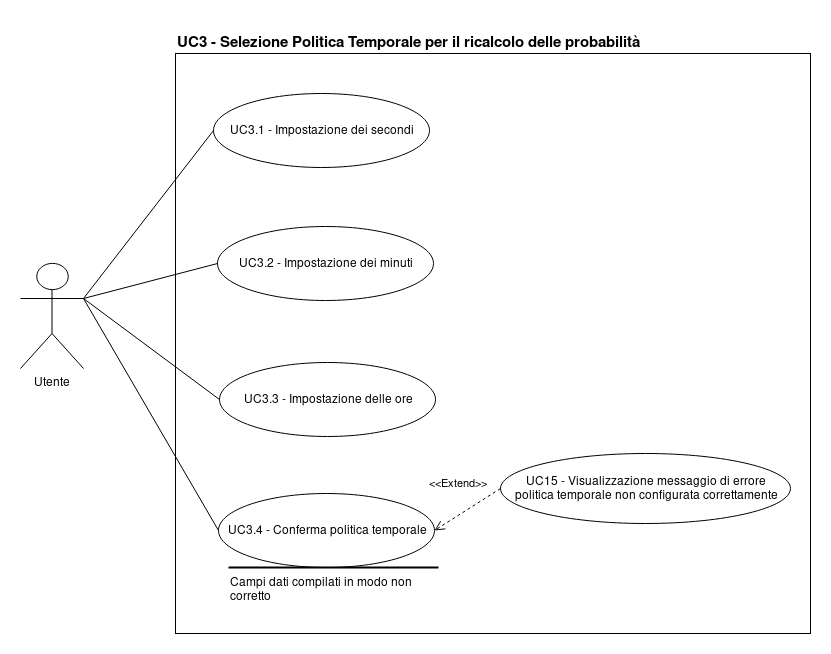
\includegraphics[scale=0.5]{./images/UC3.png}
\caption{UC3 - Selezione Politica Temporale di Ricalcolo delle Probabilità.}
\end{figure}

\begin{itemize}
	\item \textbf{Attore Primario}: Utente;
	\item \textbf{Precondizione}:
		\begin{enumerate}
			\item L'utente deve aver correttamente configurato la connessione al server (\hyperref[UC17]{UC17 (§\ref*{UC17})});
			\item L'utente si trova presso il pannello di configurazione della Politica Temporale, acceduto tramite il click del pulsante "Configurazione Politica Temporale";
			\item L'utente visualizza tre campi dati editabili, rispettivamente "secondi", "minuti" e "ore", necessari per la configurazione della politica temporale.
		\end{enumerate}
	\item \textbf{Postcondizione}: L'utente ha configurato con successo la politica temporale da lui creata, per il ricalcolo delle probabilità della rete bayesiana, caricata in (\hyperref[UC1]{UC1 (§\ref*{UC1})});
	\item \textbf{Scenario Principale:}
	\begin{enumerate}
		\item (\hyperref[UC3.1]{UC3.1 (§\ref*{UC3.1})}) Impostazione dei secondi;
		\item (\hyperref[UC3.2]{UC3.2 (§\ref*{UC3.2})}) Impostazione dei minuti;
		\item (\hyperref[UC3.3]{UC3.3 (§\ref*{UC3.3})}) Impostazione delle ore;
		\item (\hyperref[UC3.4]{UC3.4 (§\ref*{UC3.4})}) Conferma della politica temporale realizzata.
	\end{enumerate}
	\item \textbf{Estensioni:} \hyperref[UC15]{UC15 (§\ref*{UC15})} estende \hyperref[UC3.4]{UC3.4 (§\ref*{UC3.4})}: l'utente visualizza un messaggio di errore nel caso in cui non abbia definito correttamente la politica temporale per il ricalcolo delle probabilità;
	\item \textbf{Inclusioni:} \hyperref[UC3]{UC3 (§\ref*{UC3})} include \hyperref[UC32]{UC32 (§\ref*{UC32})}: Viene visualizzata una notifica di avvenuta selezione della politica temporale per il ricalcolo delle probabilità.
\end{itemize}

\pagebreak

\subsubsection{UC3.1 - Impostazione dei Secondi}\label{UC3.1}

\begin{itemize}
	\item \textbf{Attore Primario}: Utente;
	\item \textbf{Precondizione}: l'utente ha acceduto al pannello di creazione della politica temporale tramite il pulsante "Configurazione Politica Temporale";
	\item \textbf{Postcondizione}: l'utente ha impostato il numero di secondi di cui è composta la politica temporale;
	\item \textbf{Scenario Principale:} l'utente edita il campo dati "secondi" inserendo il numero di secondi di cui è composta la politica temporale.
\end{itemize}

\subsubsection{UC3.2 - Impostazione dei Minuti}\label{UC3.2}

\begin{itemize}
	\item \textbf{Attore Primario}: Utente;
	\item \textbf{Precondizione}: l'utente ha acceduto al pannello di creazione della politica temporale tramite il pulsante "Configurazione Politica Temporale";
	\item \textbf{Postcondizione}: l'utente ha impostato il numero di minuti di cui è composta la politica temporale;
	\item \textbf{Scenario Principale:} l'utente edita il campo dati "minuti" inserendo il numero di minuti di cui è composta la politica temporale.
\end{itemize}


\subsubsection{UC3.3 - Impostazione delle Ore}\label{UC3.3}

\begin{itemize}
	\item \textbf{Attore Primario}: Utente;
	\item \textbf{Precondizione}: l'utente ha acceduto al pannello di creazione della politica temporale tramite il pulsante "Configurazione Politica Temporale";
	\item \textbf{Postcondizione}: l'utente ha impostato il numero delle ore di cui è composta la politica temporale;
	\item \textbf{Scenario Principale:} l'utente edita il campo dati "ore" inserendo il numero di ore di cui è composta la politica temporale.
\end{itemize}


\subsubsection{UC3.4 - Conferma Politica Temporale}\label{UC3.4}
\begin{itemize}
	\item \textbf{Attore Primario}: Utente;
	\item \textbf{Precondizione}: l'utente ha acceduto al pannello di creazione della politica temporale tramite il pulsante "Configurazione Politica Temporale";
	\item \textbf{Postcondizione}: l'utente ha confermato la politica temporale per il ricalcolo delle probabilità;
	\item \textbf{Scenario Principale}: l'utente conferma le impostazioni di definizione della politica temporale cliccando il pusante "Conferma".
	\item \textbf{Estensioni}: \hyperref[UC15]{UC15 (§\ref*{UC15})}: l'utente visualizza un messaggio di errore nel caso in cui non abbia collegato alcun nodo ad un flusso dati.
\end{itemize}

\newpage

\subsection{UC4 - Visualizzazione Probabilità Associate ai Nodi di una Rete Bayesiana Monitorata}\label{UC4}

\begin{itemize}
	\item \textbf{Attore Primario:} Utente;
	\item \textbf{Precondizioni:}
	\begin{enumerate}
 		\item L'utente ha avviato correttamente il monitoraggio del flusso dati (\hyperref[UC20]{UC20 (§\ref*{UC20})}) di una rete bayesiana;
 		\item L'utente ha selezionato la rete bayesiana di cui desidera visualizzare i dati di monitoraggio (\hyperref[UC36]{UC36 (§\ref*{UC36})}).
	\end{enumerate}
	\item \textbf{Postcondizione:} il Sistema mantiene aggiornate e visualizzabili da parte dell'utente, le misure di probabilità derivate dai nodi della rete bayesiana monitorata selezionata;
	\item \textbf{Scenario Principale:} l'utente visualizza l'andamento delle probabilità dinamiche associate ai nodi della rete bayesiana. Il sistema aggiorna costantemente i dati forniti dalla rete bayesiana, effettuando l'operazione di ricalcolo delle probabilità associate ai nodi della rete non collegati al flusso dati. Tale operazione di ricalcolo delle probabilità viene eseguita allo scadere del timeout ciclico rappresentato dalla politica temporale stabilita in \hyperref[UC3]{UC3 (§\ref*{UC3})}, oppure, nel caso siano state definite in sede di collegamento nodi (\hyperref[UC2.4.4]{UC2.4.4 (§\ref*{UC2.4.4})}), ogni volta che una soglia critica viene attivata dai dati monitorati.
\end{itemize}

\pagebreak

\subsection{UC8 - Visualizzazione Messaggio d'Errore Selezione Rete Bayesiana}\label{UC8}
\begin{itemize}
\item \textbf{Attore Primario}: Utente;
\item \textbf{Precondizione}: l'utente ha selezionato una rete da aggiungere ed ha cliccato il pulsante "Aggiungi", per confermare la rete. La rete selezionata dall'utente è errata per formato o per struttura;
\item \textbf{Postcondizione}: l'utente visualizza l'errore, viene quindi riportato alla finestra di selezione del file della rete bayesiana (\hyperref[UC1.2]{UC1.2 (§\ref*{UC1.2})});
\item \textbf{Scenario Principale:}
	\begin{enumerate}
	\item L'utente visualizza un messaggio di errore in cui è segnalato il fatto che la struttura del file di definizione della rete bayesiana, caricato in (\hyperref[UC1.2]{UC1.2 (§\ref*{UC1.2})}, non è corretta;
	\item L'utente clicca il pulsante con etichetta "OK".
	\end{enumerate}
\end{itemize}

\pagebreak

\subsection{UC9 - Visualizzazione Messaggio di Errore Nessun Nodo Collegato}\label{UC9}
\begin{itemize}
\item \textbf{Attore Primario}: Utente;
\item \textbf{Precondizione}: l'utente ha avviato il monitoraggio (\hyperref[UC20]{UC20 (§\ref*{UC20})}), senza averne effettivamente collegato alcuno;
\item \textbf{Postcondizioni}:
	\begin{enumerate}
	\item L'utente visualizza l'errore;
	\item Il monitoraggio dei dati non viene avviato.
	\end{enumerate}
\item \textbf{Scenario Principale}:
	\begin{enumerate}
	\item L'utente visualizza un messaggio di errore in cui è segnalato il fatto che non sia stato collegato alcun 				nodo al flusso dati (\hyperref[UC2]{UC2 (§\ref*{UC2})});
	\item L'utente clicca il pulsante con etichetta "OK".
	\end{enumerate}
\end{itemize}

\pagebreak

\subsection{UC12 - Visualizzazione Messaggio di Errore Politica Temporale non Definita}\label{UC12}
\begin{itemize}
\item \textbf{Attore Primario}: Utente;
\item \textbf{Precondizione}: l'utente ha avviato il monitoraggio del flusso dati (\hyperref[UC20]{UC20 							(§\ref*{UC20})}), senza aver preventivamente definito correttamente alcuna politica temporale per il ricalcolo delle probabilità (\hyperref[UC3]{UC3 (§\ref*{UC3})}).
\item \textbf{Postcondizione}: l'utente visualizza l'errore;
\item \textbf{Scenario Principale}:
	\begin{enumerate}
	\item L'utente visualizza un messaggio di errore in cui è segnalato il fatto che non sia stata definita alcuna 				politica temporale per il ricalcolo delle probabilità;
	\item L'utente clicca il pulsante con etichetta "OK".
	\end{enumerate}
\end{itemize}

\newpage

\subsection{UC14 - Visualizzazione Messaggio di Errore Impostazioni di Collegamento}\label{UC14}
\begin{itemize}
\item \textbf{Attore Primario}: Utente;
\item \textbf{Precondizione}: l'utente ha confermato le scelte per il collegamento di un dato nodo ad un flusso dati (\hyperref[UC2.6]{UC2.6 (§\ref*{UC2.6})}), avendo commesso alcuni errori durante la definizione delle impostazioni di collegamento;
\item \textbf{Postcondizioni}:
	\begin{enumerate}
	\item L'utente visualizza l'errore;
	\item Le scelte dell'utente non vengono confermate.
	\end{enumerate}
\item \textbf{Scenario Principale}:
	\begin{enumerate}
	\item L'utente visualizza un messaggio di errore in cui sono indicati gli errori commessi;
	\item L'utente clicca il pulsante con etichetta "OK".
	\end{enumerate}
\end{itemize}

\pagebreak

\subsection{UC15 - Visualizzazione Messaggio di Errore Politica Temporale non Configurata Correttamente}\label{UC15}
\begin{itemize}
	\item \textbf{Attore Primario}: Utente;
	\item \textbf{Precondizione}: l'utente ha confermato le scelte per la selezione di una politica temporale per il ricalcolo delle probabilità (\hyperref[UC3.4]{UC3.4 (§\ref*{UC3.4})}), senza averla definita correttamente;
	\item \textbf{Postcondizioni}:
	\begin{enumerate}
		\item L'utente visualizza il messaggio d'errore;
		\item La politica temporale non viene impostata.
	\end{enumerate}
	\item \textbf{Scenario Principale}:
	\begin{enumerate}
		\item L'utente visualizza un messaggio di errore in cui sono indicati gli errori commessi;
		\item L'utente clicca il pulsante con etichetta "OK".
	\end{enumerate}
\end{itemize}

\pagebreak

\subsection{UC16 - Visualizzazione della Lista dei Nodi della Rete Bayesiana}\label{UC16}
\begin{itemize}
	\item \textbf{Attore Primario:}  Utente;
	\item \textbf{Precondizione:} l'utente ha caricato con successo la rete bayesiana (\hyperref[UC1]{UC1 	(§\ref*{UC1})});
	\item \textbf{Postcondizione:} l'utente visualizza la lista di nodi di cui la rete bayesiana è costituita;
	\item \textbf{Scenario Principale:}
	\begin{enumerate}
		\item L'utente visualizza la lista di nodi di cui la rete bayesiana, caricata in \hyperref[UC1]{UC1 									(§\ref*{UC1})}, è costituita. Ogni elemento della lista è formato da due componenti:
		\begin{itemize}
			\item Il nominativo del nodo stesso;
			\item Una checkbox che rappresenta lo stato di collegamento del nodo a cui è associata: verrà cisualizzata una "V" nel caso il nodo sia collegato ad un flusso dati, checkbox vuota altrimenti.
		\end{itemize}
	\end{enumerate}
\end{itemize}

\pagebreak

\subsection{UC17 - Configurazione Indirizzo e Porta del Server}\label{UC17}
\begin{figure}[H]
	\centering
	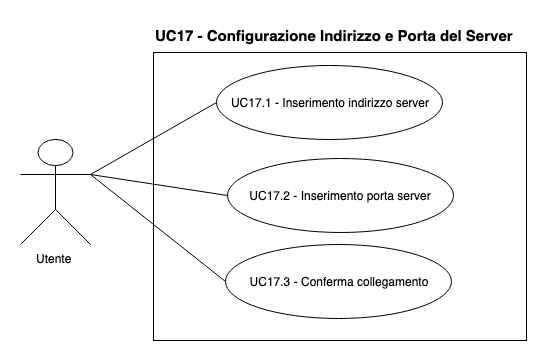
\includegraphics[scale=0.65]{./images/UC17.png}
	\caption{UC17 - Configurazione Indirizzo e Porta del Server.}
\end{figure}
\begin{itemize}
	\item \textbf{Attore Primario:}  Utente;
	\item \textbf{Precondizione:}
		\begin{enumerate}
			\item L'utente ha aggiunto il pannello \textit{G\&B} alla propria dashboard;
			\item L'utente si trova nella scheda "Server Setting" del menù "Edit" del pannello.
		\end{enumerate}
	\item \textbf{Postcondizione:} l'utente ha configurato i parametri di connessione al server atto a memorizzare le reti bayesiane caricate con le rispettive impostazioni di collegamento al flusso dati, ed eseguire i calcoli per il ricalcolo delle probabilità in sede di monitoraggio;
	\item \textbf{Scenario Principale:}
	\begin{enumerate}
		\item (\hyperref[UC17.1]{UC17.1 (§\ref*{UC17.1})}) Inserimento indirizzo IP;
		\item (\hyperref[UC17.2]{UC17.2 (§\ref*{UC17.2})}) Inserimento porta;
		\item (\hyperref[UC17.3]{UC17.3 (§\ref*{UC17.3})}) Click conferma collegamento.
	\end{enumerate}
	\item \textbf{Estensioni}: si è verificato un errore di connessione: l'utente visualizza un messaggio che lo informa dell'avvenuto errore, invitandolo quindi a verificare la correttezza di indirizzo e/o porta (\hyperref[UC22]{UC22 (§\ref*{UC22})});
	\item \textbf{Inclusioni:} UC17 include \hyperref[UC26]{UC26 (§\ref*{UC26})}: Viene visualizzata una notifica di avvenuto collegamento;
\end{itemize}

\subsubsection{UC17.1 - Inserimento Indirizzo Server}\label{UC17.1}
\begin{itemize}
	\item \textbf{Attore Primario:}  Utente
	\item \textbf{Precondizione:} l'utente si trova nella scheda "Server Setting" del menù "Edit" del pannello;
	\item \textbf{Postcondizione:} l'utente ha inserito l'indirizzo per la connessione al server;
	\item \textbf{Scenario Principale:} l'utente inserisce l'indirizzo IP del server a cui desidera collegarsi nell'apposito campo di testo.
\end{itemize}

\subsubsection{UC17.2 - Inserimento Porta Server}\label{UC17.2}
\begin{itemize}
	\item \textbf{Attore Primario:}  Utente;
	\item \textbf{Precondizione:} l'utente si trova nella scheda "Server Setting" del menù "Edit" del pannello;
	\item \textbf{Postcondizione:} l'utente ha inserito il numero della porta per la connessione al server;
	\item \textbf{Scenario Principale:} l'utente inserisce il numero della porta del server a cui desidera collegarsi nell'apposito campo di testo.
\end{itemize}

\subsubsection{UC17.3 - Conferma Collegamento}\label{UC17.3}
\begin{itemize}
	\item \textbf{Attore Primario:}  Utente;
	\item \textbf{Precondizione:} l'utente si trova nella scheda "Server Setting" del menù "Edit" del pannello;
	\item \textbf{Postcondizione:} l'utente ha confermato i parametri inseriti precedentemente per la connessione al server;
	\item \textbf{Scenario Principale:} l'utente clicca il pulsante con etichetta "Collega".
\end{itemize}

\pagebreak

\subsection{UC18 - Selezione Database}\label{UC18}
\begin{itemize}
	\item \textbf{Attore Primario:} Utente;
	\item \textbf{Precondizione:} l'utente ha correttamente configurato le impostazioni per la connessione al server \hyperref[UC17]{UC17(§\ref*{UC17})};
	\item \textbf{Postcondizioni:}
	\begin{enumerate}
		\item L'utente ha selezionato il database da usare come sorgente dati;
		\item Contestualmente al database selezionato dall'utente, cambiano le possibili scelte in sede di collegamento nodi (\hyperref[UC2]{UC2(§\ref*{UC2})}), per la selezione della tabella (\hyperref[UC2.2]{UC2.2(§\ref*{UC2.2})}) e del flusso dati (\hyperref[UC2.3]{UC2.3(§\ref*{UC2.3})}).
	\end{enumerate}
	\item \textbf{Scenario Principale:} l'utente seleziona, attraverso un menù a tendina, il database da usare come sorgente dati tra quelli disponibili;
	\item \textbf{Inclusioni:} UC18 include (\hyperref[UC31]{UC31(§\ref*{UC31})}): Viene visualizzata una notifica di avvenuta selezione del database.
\end{itemize}

\pagebreak

\subsection{UC19 - Scollegamento Nodo}\label{UC19}
\begin{itemize}
	\item \textbf{Attore Primario:} Utente;
	\item \textbf{Precondizione:} l'utente ha confermato il collegamento del nodo (\hyperref[UC2.6]{UC2.6 									(§\ref*{UC2.6})});
	\item \textbf{Postcondizioni:}
	\begin{enumerate}
		\item L'utente ha scollegato il nodo dal flusso dati;
		\item Il Sistema aggiorna la checkbox del nodo, togliendo la spunta che indica il collegamento;
		\item Il pulsante "Scollega Nodo" scompare.
	\end{enumerate}
	\item \textbf{Scenario Principale:} l'utente scollega il nodo collegato desiderato, cliccando il pulsante "Scollega Nodo" accanto al nominativo dello stesso.
\end{itemize}

\pagebreak

\subsection{UC20 - Avvio Monitoraggio}\label{UC20}

\begin{itemize}
	\item \textbf{Attore Primario:} Utente;
	\item \textbf{Precondizione:} l'utente ha caricato con successo la rete bayesiana (\hyperref[UC1]{UC1(§\ref*{UC1})});
	\item \textbf{Postcondizioni:}
	\begin{enumerate}
		\item Il pulsante "Avvio Monitoraggio" viene sostituito da "Interruzione Monitoraggio";
		\item La rete bayesiana, con le corrispondenti impostazioni di collegamento, viene salvata nel server. Tale rete potrà dunque essere selezionata dall'utente durante \hyperref[UC23]{UC23(§\ref*{UC23})};
		\item L'utente non ha più la possibilità di modificare le impostazioni di collegamento della rete di cui ha avviato il monitoraggio, può però selezionare una rete differente (\hyperref[UC23]{UC23(§\ref*{UC23})}) oppure caricarne una nuova (\hyperref[UC23]{UC23(§\ref*{UC23})}).
	\end{enumerate}
	\item \textbf{Scenario Principale:} l'utente avvia il monitoraggio cliccando il pulsante denominato "Avvio Monitoraggio". Questo porta all'invio della configurazione della rete bayesiana (stabilita dall'utente attraverso \hyperref[UC1]{UC1 (§\ref*{UC1})}, \hyperref[UC2]{UC2 (§\ref*{UC2})}, \hyperref[UC18]{UC18 (§\ref*{UC18})} e \hyperref[UC3]{UC3 (§\ref*{UC3})}) al Server (in ascolto presso la porta stabilita dall'utente in \hyperref[UC17]{UC17 (§\ref*{UC17})}) che si occuperà delle necessarie operazioni per gestire il monitoraggio dei dati.
	\item \textbf{Estensioni:}
	\begin{enumerate}
		\item \hyperref[UC9]{UC9 (§\ref*{UC9})}: l'utente visualizza un messaggio di errore nel caso in cui non abbia collegato alcun nodo ad un flusso dati (\hyperref[UC2]{UC2 (§\ref*{UC2})});
		\item \hyperref[UC12]{UC12 (§\ref*{UC12})}: l'utente visualizza un messaggio di errore nel caso in cui non abbia definito correttamente alcuna politica temporale per il ricalcolo delle probabilità (\hyperref[UC3]{UC3 (§\ref*{UC3})}).
	\end{enumerate}
	\item \textbf{Inclusioni:} UC20 include \hyperref[UC34]{UC34 (§\ref*{UC34})}: Viene visualizzato nel pannello una notifica di avvio monitoraggio della rete bayesiana.
\end{itemize}

\pagebreak

\subsection{UC21 - Interruzione Monitoraggio}\label{UC21}

\begin{itemize}
	\item \textbf{Attore Primario:} Utente;
	\item \textbf{Precondizione:}
	\begin{enumerate}
		\item L'utente ha aggiunto il pannello \textit{G\&B} alla propria dashboard;
		\item L'utente ha avviato il monitoraggio (\hyperref[UC20]{UC20(§\ref*{UC20})}).
	\end{enumerate}
	\item \textbf{Postcondizione:} l'utente ha interrotto il monitoraggio precedentemente attivo;
	\item \textbf{Scenario Principale:} l'utente interrompe il monitoraggio della rete le cui impostazioni sono attualmente visualizzate attraverso il click del bottone con etichetta "Interrompi Monitoraggio";
	\item \textbf{Inclusioni:} UC21 include \hyperref[UC35]{UC35 (§\ref*{UC35})}: Viene visualizzato nel pannello una notifica di avvio monitoraggio della rete bayesiana.
\end{itemize}

\pagebreak

\subsection{UC22 - Visualizzazione Errore nel Collegamento al Server}\label{UC22}
%\begin{figure}[H]
%	\centering
%	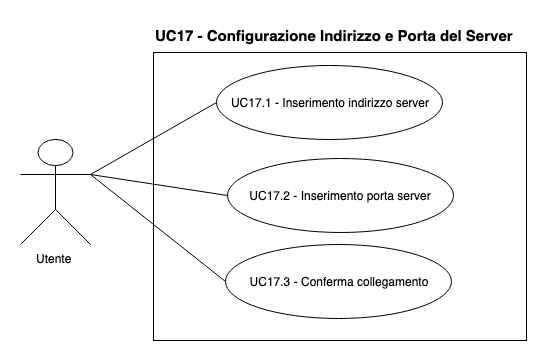
\includegraphics[scale=0.5]{./images/UC17.png}
%	\caption{UC17 - Configurazione Indirizzo e Porta del Server.}
%\end{figure}
\begin{itemize}
	\item \textbf{Attore Primario:}  Utente;
	\item \textbf{Precondizione:} l'utente ha cliccato il pulsante con etichetta "Collega" per confermare il collegamento al server (\hyperref[UC17]{UC17 (§\ref*{UC17})}) commettendo degli errori;
	\item \textbf{Postcondizione:} l'utente ha visualizzato il messaggio di errore;
	\item \textbf{Scenario Principale:}
	\begin{enumerate}
		\item L'utente visualizza il messaggio che notifica gli errori commessi;
		\item L'utente clicca "OK".
	\end{enumerate}
\end{itemize}

\pagebreak

\subsection{UC23 - Selezione Rete Bayesiana già Caricata}\label{UC23}
\begin{itemize}
	\item \textbf{Attore Primario:}  Utente;
	\item \textbf{Precondizione:} l'utente ha correttamente configurato le impostazioni per la connessione al server (\hyperref[UC17]{UC17(§\ref*{UC17})});
	\item \textbf{Postcondizione:}
	\begin{enumerate}
		\item L'utente visualizza le impostazioni della rete selezionata;
		\item Le eventuali impostazioni di rete, visualizzate prima del cambio, vengono salvate nel server come rete già caricata.
	\end{enumerate}
	\item \textbf{Scenario Principale:} l'utente, attraverso un menù a tendina, seleziona una rete bayesiana (con eventuali relative impostazioni di collegamento) tra quelle già caricate e/o correntemente monitorate, e quindi salvate nel server.
\end{itemize}

\pagebreak

\subsection{UC24 - Visualizzazione Monitoraggi Attivi}\label{UC24}
\begin{itemize}
	\item \textbf{Attore Primario:}  Utente;
	\item \textbf{Precondizioni:} 
	\begin{enumerate}
		\item L'utente deve aver effettuato il login nella piattaforma \textit{Grafana}, deve aver selezionato una dashboard e aggiunto il pannello \textit{G\&B};
		\item L'utente deve aver correttamente configurato la connessione al server (\hyperref[UC17]{UC17 (§\ref*{UC17})}).
	\end{enumerate}
	\item \textbf{Postcondizione:} la vista del plug-in, contentente le impostazioni di collegamento di una rete bayesiana, viene sostituita da una sezione atta alla visualizzazione dei monitoraggi attivi;
	\item \textbf{Scenario Principale:} l'utente per accedere alla visualizzazione dei monitoraggi attivi, clicca il pulsante con etichetta "Visualizzazione monitoraggio".
\end{itemize}

\pagebreak

\subsection{UC25 - Visualizzazione Impostazioni di Collegamento}\label{UC25}
\begin{itemize}
	\item \textbf{Attore Primario:} Utente;
	\item \textbf{Precondizione:} 
	\begin{enumerate}
		\item L'utente deve aver effettuato il login nella piattaforma \textit{Grafana}, deve aver selezionato una dashboard e aggiunto il pannello \textit{G\&B};
		\item L'utente deve aver correttamente configurato la connessione al server (\hyperref[UC17]{UC17 (§\ref*{UC17})});
		\item L'utente sta visualizzando i monitoraggi attivi.
	\end{enumerate}
	\item \textbf{Postcondizione:} La sezione del plug-in, atta alla visualizzazione dei monitoraggi attivi, viene sostituita dalle impostazioni di collegamento della rete bayesiana;
	\item \textbf{Scenario Principale:} l'utente per accedere alla visualizzazione delle impostazioni di collegamento, clicca il pulsante con etichetta "Visualizzazione impostazioni collegamento".
\end{itemize}

\pagebreak

\subsection{UC26 - Visualizzazione Notifica di Avvenuto Collegamento al Server}\label{UC26}

\begin{itemize}
	\item \textbf{Attore Primario:}  Utente;
	\item \textbf{Precondizione:} l'utente ha cliccato il pulsante con etichetta "Collega" per confermare il collegamento al server con i dati precedentemente impostati (\hyperref[UC17]{UC17 (§\ref*{UC17})});
	\item \textbf{Postcondizione:} l'utente visualizza la notifica dell'avvenuto collegamento;
	\item \textbf{Scenario Principale:}
	\begin{enumerate}
		\item L'utente visualizza il messaggio dell'avvenuto collegamento;
		\item L'utente clicca "OK".
	\end{enumerate}
\end{itemize}

\pagebreak

\subsection{UC27 - Rimozione Rete Bayesiana}\label{UC27}

\begin{itemize}
	\item \textbf{Attore Primario:} Utente;
	\item \textbf{Precondizioni:}
	\begin{enumerate}
 		\item L'utente ha correttamente configurato le impostazioni per la connessione al server (\hyperref[UC17]{UC17(§\ref*{UC17})});
 		\item L'utente ha precedentemente caricato una rete bayesiana (\hyperref[UC1]{UC1(§\ref*{UC1})}).
	\end{enumerate}
	\item \textbf{Postcondizione:} l'utente ha eliminato la rete bayesiana selezionata;
	\item \textbf{Scenario Principale:}
	\begin{enumerate}
		\item L'utente seleziona la rete bayesiana, tra quelle memorizzate nel server, che desidera eliminare attraverso un menù a tendina;
		\item L'utente rimuove la rete bayesiana selezionata cliccando il tasto "Elimina".
	\end{enumerate}
	\item \textbf{Estensioni:} \hyperref[UC28]{UC28 (§\ref*{UC28})}: l'utente visualizza un messaggio di errore nel caso in cui abbia tentato di rimuovere una rete bayesiana in monitoraggio.
	\item \textbf{Inclusioni:} UC27 include \hyperref[UC29]{UC29 (§\ref*{UC29})}: l'utente visualizza una notifica di avvenuta rimozione della rete bayesiana.
\end{itemize}

\pagebreak

\subsection{UC28 - Visualizzazione Messaggio d'Errore Rimozione Rete Bayesiana}\label{UC28}

\begin{itemize}
	\item \textbf{Attore Primario:} Utente;
	\item \textbf{Precondizione:} l'utente ha tentato di rimuovere una rete bayesiana (\hyperref[UC27]{UC27(§\ref*{UC27})}) in monitoraggio attivo;
	\item \textbf{Postcondizioni:}
	\begin{enumerate}
		\item L'utente visualizza il messaggio di errore;
		\item La rimozione della rete bayesiana viene annullata.
	\end{enumerate}
	\item \textbf{Scenario Principale:}
	\begin{enumerate}
		\item L'utente visualizza un messaggio di errore in cui è segnalato il fatto che ha tentato di rimuovere una rete bayesiana in fase monitoraggio attivo. All'utente viene segnalata la necessità di interrompere preventivamente il monitoraggio (\hyperref[UC21]{UC21(§\ref*{UC21})}) prima di procedere con la rimozione della rete (\hyperref[UC27]{UC27(§\ref*{UC27})});
		\item L'utente clicca il pulsante con etichetta "OK".
	\end{enumerate}
\end{itemize}

\pagebreak

\subsection{UC29 - Visualizzazione Notifica Avvenuta Rimozione Rete Bayesiana}\label{UC29}

\begin{itemize}
	\item \textbf{Attore Primario:} Utente;
	\item \textbf{Precondizione:} l'utente ha rimosso una rete bayesiana tra quelle memorizzate nel server (\hyperref[UC27]{UC27(§\ref*{UC27})});
	\item \textbf{Postcondizione:} L'utente visualizza la notifica di avvenuta rimozione;
	\item \textbf{Scenario Principale:}
	\begin{enumerate}
		\item L'utente visualizza il messaggio dell'avvenuta rimozione della rete bayesiana;
		\item L'utente clicca "OK".
	\end{enumerate}
\end{itemize}

\pagebreak

\subsection{UC30 - Visualizzazione Notifica Avvenuto Caricamento Rete Bayesiana}\label{UC30}

\begin{itemize}
	\item \textbf{Attore Primario:} Utente;
	\item \textbf{Precondizione:} l'utente ha caricato una rete bayesiana (\hyperref[UC1]{UC1(§\ref*{UC1})});
	\item \textbf{Postcondizione:} l'utente visualizza la notifica di avvenuto caricamento;
	\item \textbf{Scenario Principale:}
	\begin{enumerate}
		\item L'utente visualizza il messaggio dell'avvenuto caricamento della rete bayesiana;
		\item L'utente clicca "OK".
	\end{enumerate}
\end{itemize}

\pagebreak

\subsection{UC31 - Visualizzazione Notifica Avvenuta Selezione Database}\label{UC31}

\begin{itemize}
	\item \textbf{Attore Primario:} Utente;
	\item \textbf{Precondizione:} l'utente ha selezionato il database da usare come sorgente dati (\hyperref[UC18]{UC18(§\ref*{UC18})});
	\item \textbf{Postcondizione:} l'utente visualizza la notifica di avvenuta selezione del database;
	\item \textbf{Scenario Principale:}
	\begin{enumerate}
		\item L'utente visualizza il messaggio che notifica l'avvenuta selezione del database da usare come sorgente dati;
		\item L'utente clicca "OK".
	\end{enumerate}
\end{itemize}

\pagebreak

\subsection{UC32 - Visualizzazione Notifica Avvenuta Selezione Politica Temporale}\label{UC32}

\begin{itemize}
	\item \textbf{Attore Primario:} Utente;
	\item \textbf{Precondizione:} l'utente ha impostato una politica temporale (\hyperref[UC3]{UC3(§\ref*{UC3})});
	\item \textbf{Postcondizione:} l'utente visualizza la notifica di avvenuta selezione della politica temporale per il ricalcolo delle probabilità;
	\item \textbf{Scenario Principale:}
	\begin{enumerate}
		\item L'utente visualizza il messaggio che notifica l'avvenuta selezione della politica temporale di ricalcolo delle probabilità;
		\item L'utente clicca "OK".
	\end{enumerate}
\end{itemize}

\pagebreak

\subsection{UC33 - Visualizzazione Notifica Avvenuto Collegamento Nodo}\label{UC33}

\begin{itemize}
	\item \textbf{Attore Primario:} Utente;
	\item \textbf{Precondizione:} l'utente ha confermato le impostazioni di collegamento di un nodo (\hyperref[UC2.6]{UC2.6 (§\ref*{UC2.6})});
	\item \textbf{Postcondizione:} l'utente visualizza la notifica di avvenuto collegamento del nodo al flusso dati;
	\item \textbf{Scenario Principale:}
	\begin{enumerate}
		\item L'utente visualizza il messaggio che notifica l'avvenuto collegamento al flusso dati di un nodo della rete bayesiana (caricata in \hyperref[UC1]{UC1 (§\ref*{UC1})});
		\item L'utente clicca "OK".
	\end{enumerate}
\end{itemize}

\pagebreak

\subsection{UC34 - Visualizzazione Notifica Monitoraggio Avviato}\label{UC34}

\begin{itemize}
	\item \textbf{Attore Primario:} Utente;
	\item \textbf{Precondizione:} l'utente ha avviato il monitoraggio di una rete bayesiana (\hyperref[UC20]{UC20 (§\ref*{UC20})});
	\item \textbf{Postcondizione:} l'utente visualizza la notifica di avvio monitoraggio dati;
	\item \textbf{Scenario Principale:}
	\begin{enumerate}
		\item L'utente visualizza il messaggio che notifica l'avvio del monitoraggio per la rete bayesiana attualmente visualizzata nel pannello;
		\item L'utente clicca "OK".
	\end{enumerate}
\end{itemize}

\pagebreak

\subsection{UC35 - Visualizzazione Notifica Monitoraggio Interrotto}\label{UC35}

\begin{itemize}
	\item \textbf{Attore Primario:} Utente;
	\item \textbf{Precondizione:} l'utente ha interrotto il monitoraggio di una rete bayesiana (\hyperref[UC21]{UC21 (§\ref*{UC21})});
	\item \textbf{Postcondizione:} l'utente visualizza la notifica di interruzione del monitoraggio dati;
	\item \textbf{Scenario Principale:}
	\begin{enumerate}
		\item L'utente visualizza il messaggio che notifica l'interruzione del monitoraggio della rete bayesiana attualmente visualizzata nel pannello;
		\item L'utente clicca "OK".
	\end{enumerate}
\end{itemize}

\pagebreak

\subsection{UC36 - Selezione della Rete Bayesiana in Monitoraggio di cui Visualizzare i Dati}\label{UC36}

\begin{itemize}
	\item \textbf{Attore Primario:} Utente;
	\item \textbf{Precondizioni:} 
	\begin{enumerate}
		\item L'utente ha avviato correttamente il monitoraggio del flusso dati (\hyperref[UC20]{UC20 (§\ref*{UC20})}) di una rete bayesiana;
		\item L'utente ha effettuato l'accesso alla sezione di visualizzazione dei monitoraggi attivi (\hyperref[UC24]{UC24 (§\ref*{UC24})})
	\end{enumerate}	 
	\item \textbf{Postcondizione:} l'utente ha selezionato la rete bayesiana, tra quelle attualmente in fase di monitoraggio, di cui visualizzare i dati;
	\item \textbf{Scenario Principale:} l'utente, attraverso un menù a tendina, seleziona la rete bayesiana di cui visualizzare i dati di monitoraggio;
\end{itemize}

